%\documentclass[a4paper,10pt]{article}
%\documentclass[a4paper,10pt,landscape]{article}
\documentclass[10pt]{article}
%\usepackage[landscape, a4paper, margin=20pt]{geometry}
\usepackage[a4paper, margin=20pt]{geometry}

%\usepackage[utf8]{inputenc} 
%\usepackage[square,sort,comma,numbers]{natbib}
%\usepackage[backend=biber,autocite=inline,style=authoryear]{biblatex}
\usepackage[backend=biber,autocite=inline]{biblatex}
\addbibresource{mybib21.bib}
%\usepackage{a4wide}
\usepackage{amsmath}
\usepackage{amssymb}
\usepackage{amsthm}
\usepackage{listings}
\usepackage{color}
\usepackage{enumerate}
%\usepackage{IEEEtrantools}
%\usepackage[redeflists]{IEEEtrantools}
\usepackage{verbatim}
\usepackage{graphicx}
\usepackage{subcaption}
\usepackage[section]{placeins} %no trans-sectional figures!
\usepackage{wrapfig, framed, caption}
\usepackage{slashbox}

\usepackage{booktabs} % For \toprule, \midrule and \bottomrule
\usepackage{siunitx} % Formats the units and values
\usepackage{pgfplotstable} % Generates table from .csv
% Setup siunitx:
\sisetup{
  round-mode          = places, % Rounds numbers
  round-precision     = 2, % to 2 places
}

\usepackage{hyperref}
\hypersetup{linktocpage,
            linktoc=all,
            %colorlinks=true,
            %linkcolor=blue,
            }

\usepackage{lipsum}
%\usepackage[onehalfspace]{setspace}
\usepackage{setspace}

% Basic data
\newcommand{\N}{\mathbb{N}}
\newcommand{\C}{\mathbb{C}}
\newcommand{\ASSIGNMENT}{2}
\newcommand{\B}{\{-1,1\}}
\newcommand{\E}{\mathbf{E}}
\newcommand{\F}{\mathbb{F}}
\newcommand{\Inf}{\textbf{Inf}}
\newcommand{\I}{\mathbf{I}}
\newcommand{\NS}{\textbf{NS}}
\newcommand{\R}{\mathbb{R}}
\newcommand{\Z}{\mathbb{Z}}
\newcommand{\aufgabe}[1]{\item{\bf #1}}
\newcommand{\bvec}[1]{\mathbf{#1}}
\newcommand{\bv}[1]{\mathbf{#1}}
\newcommand{\ceil}[1]{\lceil{#1}\rceil}
\newcommand{\floor}[1]{\lfloor{#1}\rfloor}
\newcommand{\gt}{>}
\newcommand{\half}[1]{\frac{#1}{2}}
\newcommand{\lt}{<}
\newcommand{\tuple}[1]{\langle #1 \rangle}

\newcommand{\suftab}{\text{suftab}}

\setlength{\parskip}{1.0em}
\setlength{\parindent}{1em}


\lstset{
%basicstyle=\footnotesize,
%basicstyle=\ttfamily\footnotesize,
%basicstyle=\ttfamily\small,
%basicstyle=\ttfamily\scriptsize,
frame=single,
%numbers=none,
%numbersep=5pt,
numberstyle=\tiny,
showspaces=false,
showstringspaces=false,
tabsize=2,
breaklines=true,
%escapeinside={#*}{*#},
escapeinside={$}{$},
%escapeinside={*\&}{\&*},% if you want to add LaTeX within your code
%mathescape=true,
%language=C++
}

\theoremstyle{definition}
\newtheorem{mydef}{Definition}[section]

\theoremstyle{remark}
\newtheorem{remark}{Remark}

\theoremstyle{plain}
\newtheorem{thm}{Theorem}[section]
%\newtheorem{thm}{Theorem}[mydef]
\newtheorem{lemma}{Lemma}[section]
%\newtheorem{lemma}{Lemma}[mydef]

\begin{document}
\renewcommand{\thesubsection}{\thesection.\alph{subsection}}\renewcommand{\thesubsection}{\thesection.\alph{subsection}}


% Document title
\begin{titlepage}
    \title{Stitching Chromatin Puzzle with Hi-C}
    \author{Yiftach Kolb}
    %\author{\_\_\_\_\_\_\_\_\_\_\_\_\_\_\_\_\_\_}
    \date{\today}
\end{titlepage}

\maketitle

\section{Main Assumptions and Ideas}

\begin{itemize}
\item{} Two blocks of the Hi-C matrix that should be aligned
together create a pattern that 'looks right', and when they shouldn't
be adjacent or adjacent in the wrong orientation/side it 'looks
wrong'.

\item{} If we could indeed say whether every pair should(n't) be
adjacent, we can patch together the chromosome using a greedy
algorithm. This turns reduces the problem from a hard TSP situation
to an $O(n^2)$.

\item{} How do we achieve step 1? We can come up with a good 
scorign scheme to serve as a distance 'metric' or something. But
probably a better way is to train a classifier.

\item{} The Classifier. Maybe any classifier can do the job but
remember that Hi-C matrices are basically images $\Rightarrow$ NN or
some similar ML technique are very good at image classification.

\item{} What do we traim/test on? Take HI-C that that is correct,
cut it to pieces. We know the order of the pieces so we can train a
classifier to predict if two pieces belong.

\item{} Basically we rearrange blocks of the Hi-C matrix. Cut
portions (probably along the diagonal) and feed this to the NN to
train on.


\end{itemize}


\subsection{}


%\begin{figure}[htb!]
%\begin{framed}
%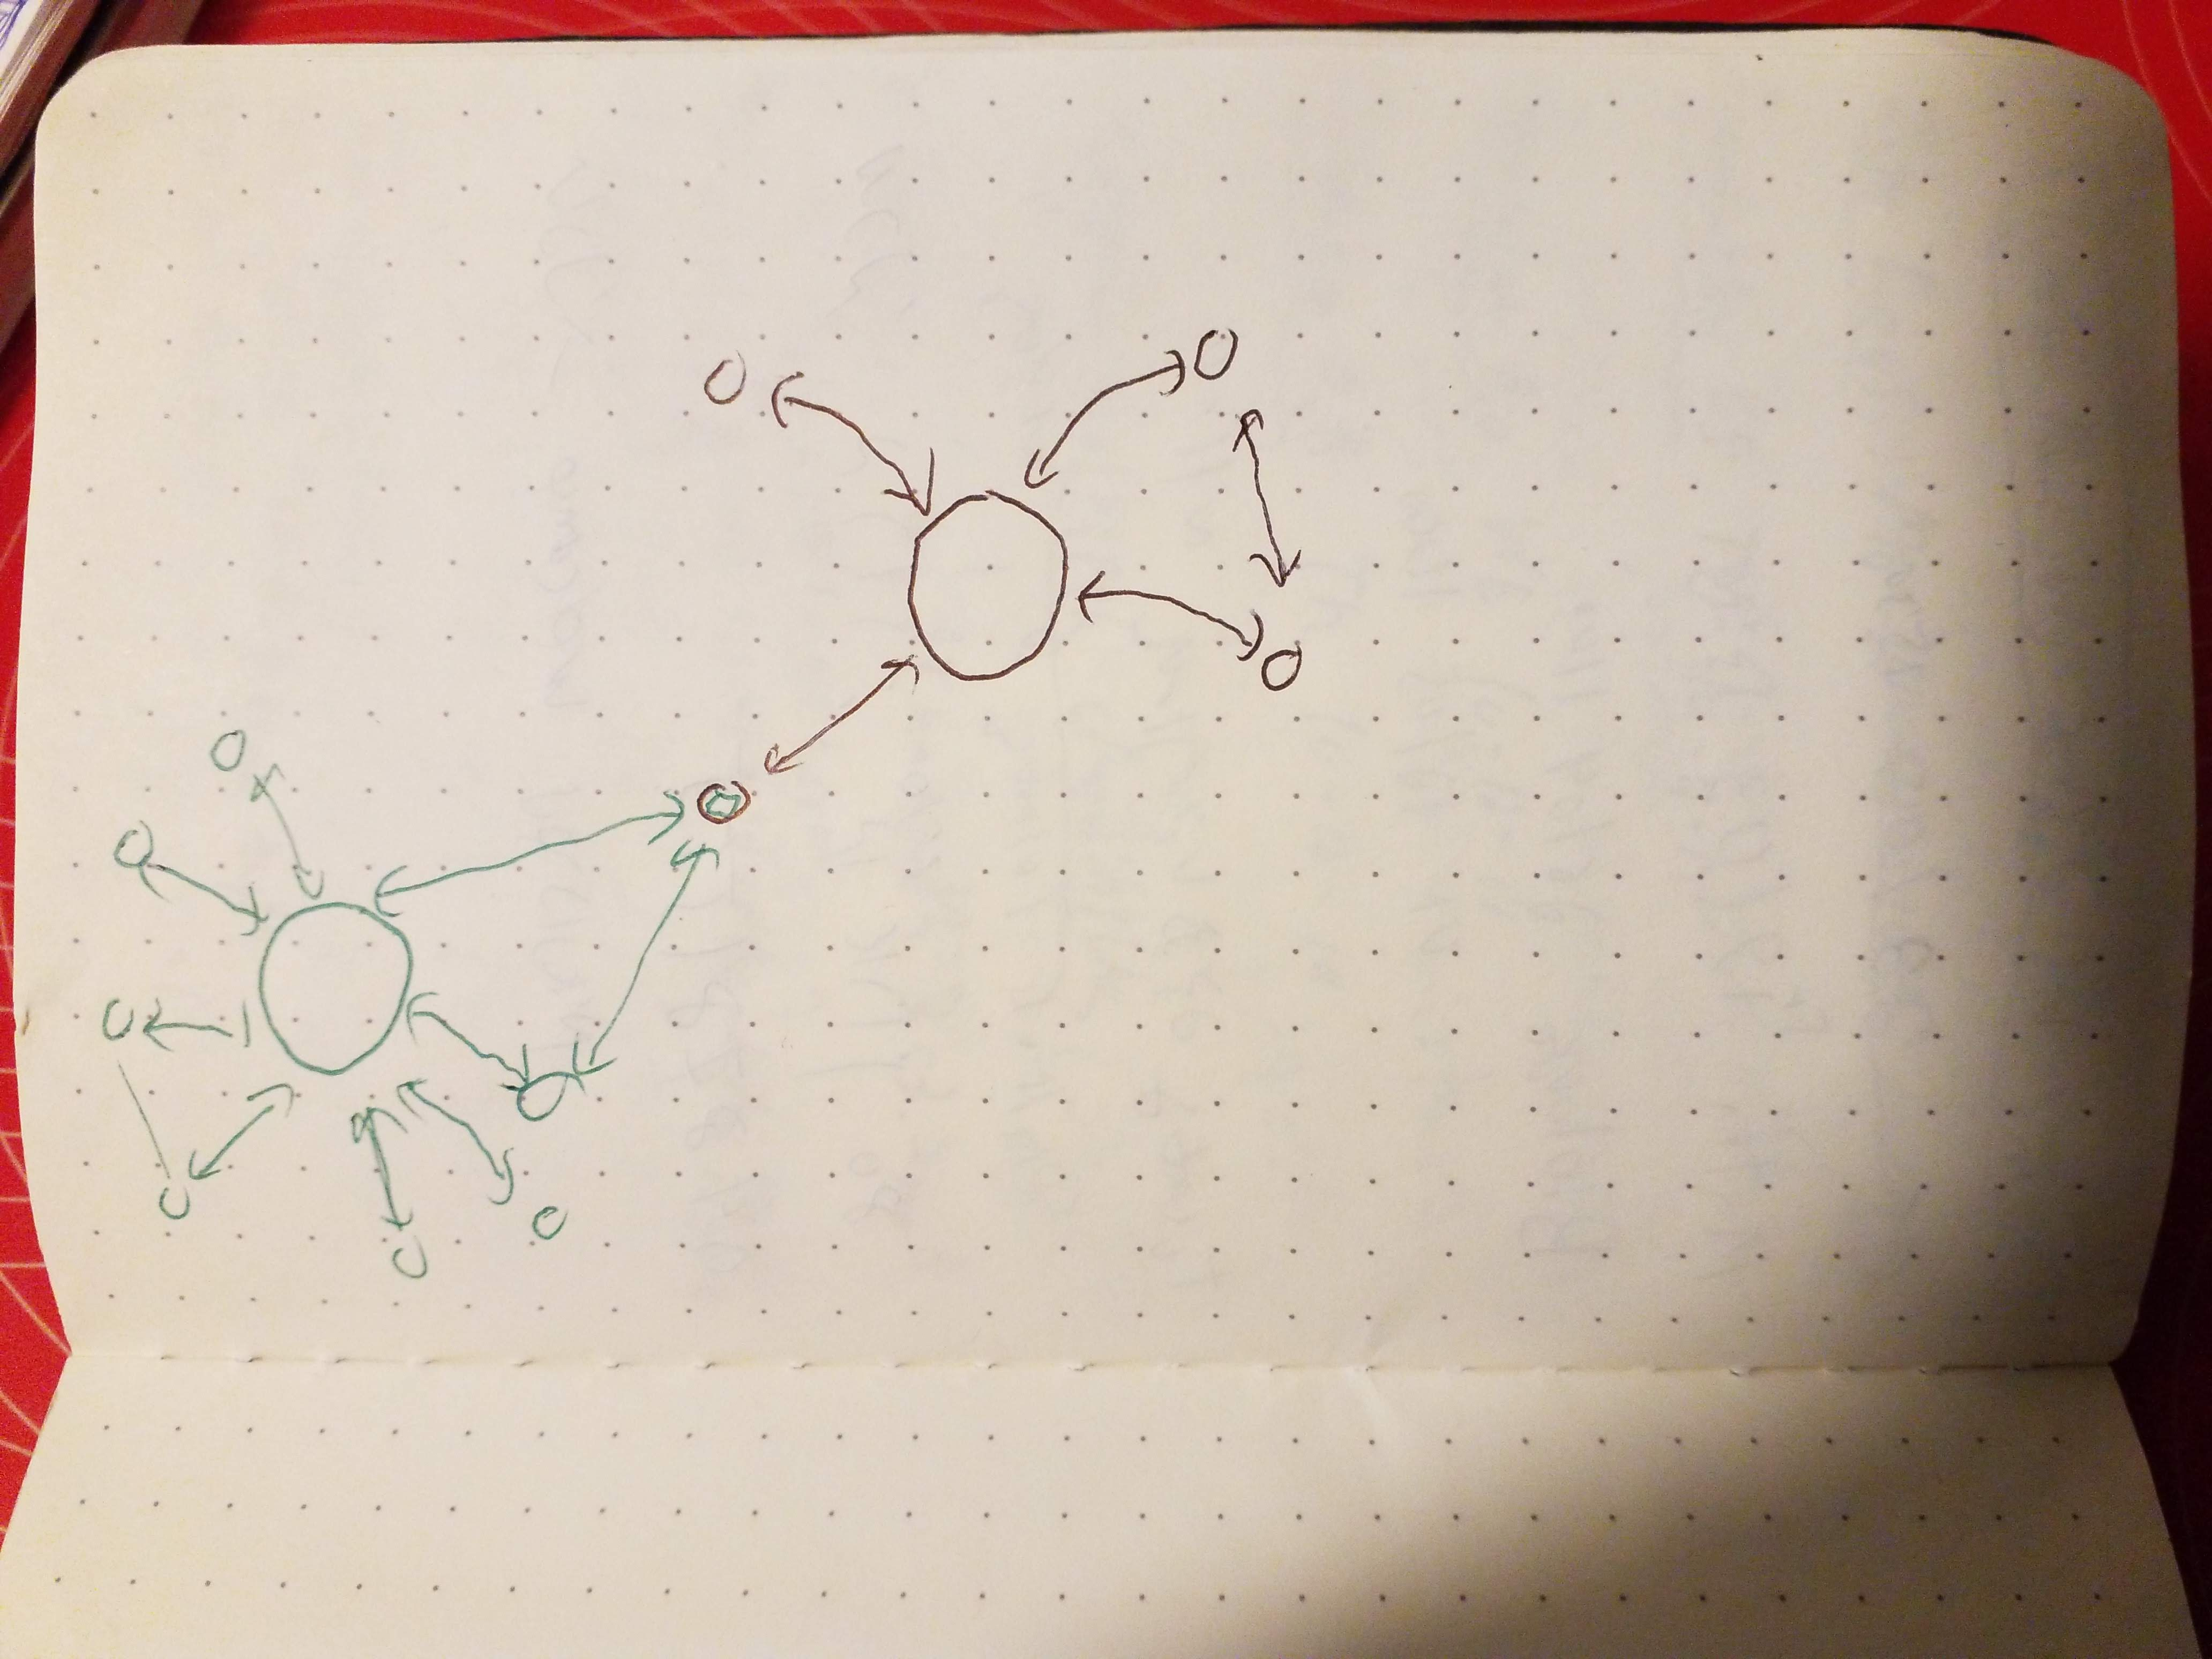
\includegraphics[width=\textwidth]{./images/plot00.jpg}
%\caption{Example where ranking fails but scoring works}
%\label{fig:rankvsscore}
%\end{framed}
%\end{figure}



% references
\section{Reference}
%\nocite{zhao2020npf}




\printbibliography

\listoffigures
\listoftables



\end{document}

